\chapter{目标代码生成}

前面的章节中,我们已经建构了抽象语法树 (AST),并进行了类型检查。在此基础上,我们需要通过抽象语法树生成目标代码。

尽管我们的确可以从抽象语法树直接生成目标平台的代码,然而现实情况并非如此。假设我们有
$m$ 门语言,$n$ 个目标平台,那么如果采用直接生成代码,则需要写 $m\times n$
个转换程序,这对于现代编译器来说是无法承受的。但是如果我们选取一门中间语言作为转换的中转,那么我只要实现
$m$ 个从语言到中间语言的转换程序,以及 $n$ 个从中间语言到目标平台的转换程序,就可以满足需求。这样的中间语言被称为
IR (intermediate representation)。此外,对于后续的优化,也可以在 IR 上处理,这可以大大减少编译器优化工作。

本章中,我们以 LLVM Language (version 15) 为例,来展示如何从中间语言转换成目标代码。如需查看
LLVM 的完整文档,请访问 \url{https://llvm.org/docs/LangRef.html}。

\section{从抽象语法树到中间语言}

在研究如何从抽象语法树转换到中间语言前,我们先熟悉一下 LLVM 15。

\subsection{LLVM 15 环境}

\subsubsection{在线 LLVM 环境}

在学习 LLVM 的过程中,一个方便的使用环境非常重要。Godbolt (
\url{https://godbolt.org/}) 提供了几乎所有的编译器,并且可以编译到大量平台。

\begin{figure}[htb]
\centering
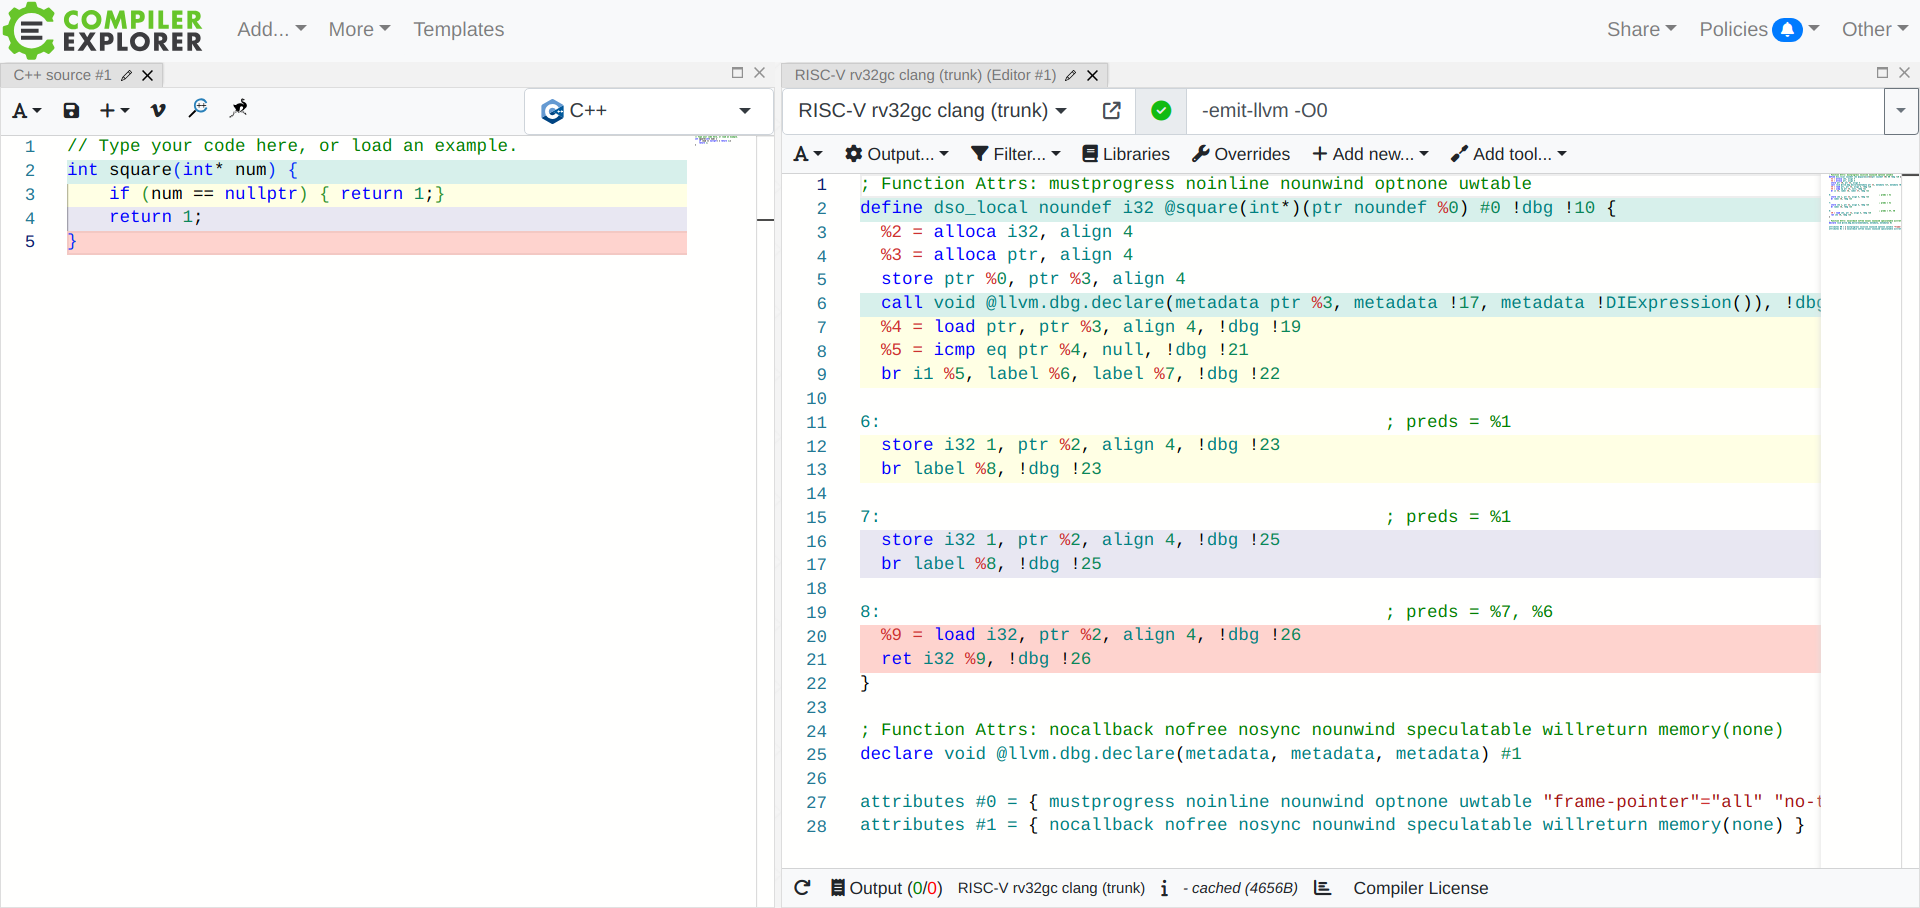
\includegraphics[scale=0.3]{image/godbolt.png}
\caption{Godbolt 使用截图}
\label{godbolt_sreenshot}
\end{figure}

图片 \ref{godbolt_sreenshot} 是一个通过在线 LLVM 环境来了解 LLVM 语言的例子。在
gofbolt 上,页面被分为两栏——左栏是你的输入,右栏是你选择的编译器在你填入的参数下的输入。下面我们将会分别介绍左右栏的使用。

左栏有一个语言选择框(位于左栏的上部)和一个代码输入框。语言选择框可以选择所使用的编程语言。

右栏上部左边部分是编译器选择框,右边部分是编译器参数框。我们此时希望将代码编译到适用于 rv32gc
平台的 LLVM 语言,而且不希望编译器做出优化(否则可能会把一部分代码直接去掉)。由于我们的编译器的目标平台是
rv32gc,且 clang 可以通过 \texttt{-emit-llvm} 来输出 LLVM 语言,因此我们在编译器选择框选择
RISCV rv32gc clang (trunk)(trunk 这里表示最新的 clang),在编译器参数框中输入 \texttt{-emit-llvm -O0}。

关于语言特性的内容,请见章节 \ref{LLVM}。

\subsubsection{本地 LLVM 环境}

你可以安装 LLVM 15 及其以上版本。截止 LLVM 17,所有的 LLVM 15 特性均可使用。

对于使用 apt 包管理的用户(debian/Ubuntu/... 用户),请参考 \href{https://apt.llvm.org/}{LLVM apt 安装文档}。

对于使用 pacman 包管理的用户,可以执行 \texttt{sudo pacman -S llvm} 安装最新版本的 LLVM。

\subsection{LLVM 15 语法}\label{LLVM}

\section{从中间语言到目标代码}

\subsection{RISC-V 汇编}

\subsection{RISC-V Calling Convention}
